\begin{itemize}
    \item Create a generative model to model the uncertainty of various scences
          \subitem i.e. Detecting weird combinations of objects within a scence
    \item Use uncertainty to make more efficient use of human labelers.
    \item Design a system which can make efficient use of uncertainty of previous stages.
\end{itemize}

Using a generative model we can generate a better explanation of why a scene is uncertain. E.g. if we are able to model the following equation:
\begin{equation}
    p(b, c, x) = p(x) * p(b | x) * p(c | x)
\end{equation}
The separate parts can be used to give a more detailed

%%------------------------------------------------------------------------------
\subsection{Motivation and Challenges}

Artificial Intelligence solutions are increasingly put in new and challenging scenarios. Yet, often AI models are only able to give a distinction between a small set of answers even when the actual answer is outside of this set \todo{Add citation} or the model has never seen anything like it before, and will gues an answer \todo{Add citation of OoD}. Uncertainty Quantification (UQ) can enable a system to detect when a prediction might be of lesser quality, and allow it to preemptively react to that. Either by stopping or requesting human intervention. Furthermore, understanding when models are uncertain, allows for more effective data sampling and labeling by making use of active learning schemes \todo{Add citations active learning usage}. The later is especially useful in industries where labeling is expensive or timeconsuming.\todo{Add citation of label cost}.

Especially in Autonomous navigation a lot of unknown objects can be present.

%%------------------------------------------------------------------------------
\subsection{Broad Literature Analysis}\label{sec:broadliterature}

This project covers broader research areas, each will be covered separately in subsections \ref{sec:broadliterature:uncertainty} and \ref{sec:broadliterature:object_detection}. Prior work in the combination will be described in subsection \ref{sec:broadliterature:combination}

\subsubsection{Uncertainty Quantification}\label{sec:broadliterature:uncertainty}
The ability to distinguish certain and uncertain outputs from machine learning models are very useful. It can be used to help decide which samples are most valuable to be manually labeled \todo{Talk about active learning}

\citep{gal2016uncertainty} distinguishes two kinds of uncertainty. Aleatoric uncertainty, the uncertainty that is caused by inprecise input data (i.e. $x$) and epistemic uncertainty, the uncertainty that is caused by the model.

Neural Networks (NN) have proven to be excelent at a broad range of tasks. However with

Uncertainty Quantification (UQ) is an important factor to increase the trust in automated processes based on machine learning. Their exist a various amount of methods both post-hoc (e.g. ) and



Reliable uncertainty estimation of Artificial Intelligence Models is important in safety critical situations. Expressing explicit uncertainty with Deep Neural Networks (DNN) can

\subsubsection{Object Detection}\label{sec:broadliterature:object_detection}


\subsubsection{In combination}\label{sec:broadliterature:combination}


%%------------------------------------------------------------------------------
\subsection{Formulation of the problem and objectives}

Include a description of the overall aim and key objectives. Explain your research questions as well as possible. Identify potential general tasks that will need to be tackled in order to complete the project successfully.

As a general rule-of-thumb, a potential evaluator would be asked to summarise the strong and weak points of the proposal as a whole. They will consider the strengths and weaknesses in such a way that they are comprehensible and substantiated for a broader scientific group. They will assess the quality, innovative character and academic impact of the proposal, including the challenging content, originality of the topic, scientific elements, potential to make an important contribution, effectiveness of proposed methodology, importance of the proposed research topic, etc.

%% THESE CITATION (nocite) ARE USED ONLY TO ILLUSTRATE THE REFERENCES. YOU SHOULD USE \cite (OR THE APPROPRIATE DERIVATION SUCH AS \citep \citet etc) WITHIN YOUR TEXT AS NEEDED
\nocite{arias2016scalable}
\nocite{batal2013efficient}
\nocite{bi2013inferring}
\nocite{bielza2011multi}

\begin{figure}[!h]
    \begin{center}

        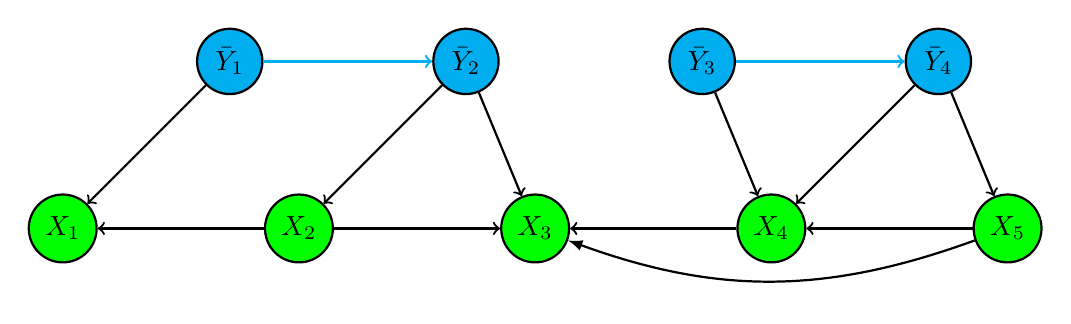
\begin{tikzpicture}[align = center, node distance=30mm, thick, main/.style = {draw, circle}]
            \node[main, fill=green] (x1) {$X_1$};
            \node[main, fill=green] (x2) [right of=x1] {$X_2$};
            \node[main, fill=green] (x3) [right of=x2] {$X_3$};
            \node[main, fill=green] (x4) [right of=x3] {$X_4$};
            \node[main, fill=green] (x5) [right of=x4] {$X_5$};
            \node[main, fill=cyan] (y1) [above right of=x1] {$\bar{Y}_1$};
            \node[main, fill=cyan] (y2) [above right of=x2] {$\bar{Y}_2$};
            \node[main, fill=cyan] (y3) [above right of=x3] {$\bar{Y}_3$};
            \node[main, fill=cyan] (y4) [above right of=x4] {$\bar{Y}_4$};
            \draw[draw=black,->] (y1) -- (x1);
            \draw[draw=black,->] (y2) -- (x2);
            \draw[draw=black,->] (y2) -- (x3);
            \draw[draw=black,->] (y3) -- (x4);
            \draw[draw=black,->] (y4) -- (x4);
            \draw[draw=black,->] (y4) -- (x5);
            \draw[draw=black,->] (x2) -- (x1);
            \draw[draw=black,->] (x2) -- (x3);
            \draw[draw=black,->] (x4) -- (x3);
            \draw[draw=black,->] (x5) -- (x4);
            \draw [draw=black,-latex] (x5) to [bend left=20] (x3);
            \draw[draw=cyan,->] (y1) -- (y2);
            \draw[draw=cyan,->] (y3) -- (y4);
        \end{tikzpicture}

        \caption{Just an example of graph using tikz, by V.L.Nguyen.}
        \label{fig:examplegraph}
    \end{center}
\end{figure}